\section{MVSNet}

	不同于传统的SfM估计一次优化能得到整个场景的点云,MVSNet\footnote{\url{https://arxiv.org/abs/1804.02505}}只是推断每张图片的深度信息,通过后处理,把多张图片的深度,拼成场景点云。\\

	主要思路是通过2张目标图来协助推断参考图的深度值,

	\begin{enumerate}
		\item 把参考相机(第一个相机)像素平面的坐标,通过192个尺度反投影到相机坐标系;然后通过单应矩阵变换到目标相机的像素坐标系。

		\small\textit{ 注意,这里的变换对象是参考相机的$120 \times 160$像素平面坐标,而非论文说的参考图像的特征图;}

		经过这步操作,可在目标相机的像素平面上形成192个$120 \times 160$的新的像素坐标值。

		\item 把投影得到的像素坐标值与目标图像的特征图结合,得到192个目标特征图

		\small\textit{把192个特征图按深度叠在一起,形成一个$192 \times 120 \times 160 \times 32$的特征图,称为\textbf{Feature Volume}}

		\item 把多个(文中为2个)目标\textbf{Feature Volume}连同参考图像的特征图一起,计算一个方差,得到的结果称为\textbf{Cost Volume},随后在\textbf{Cost Volume}上回归参考图像的深度值

		\small\textit{注意,此时才用到参考图像的特征图}
	\end{enumerate}

	\begin{figure}[H]
		\begin{center}
			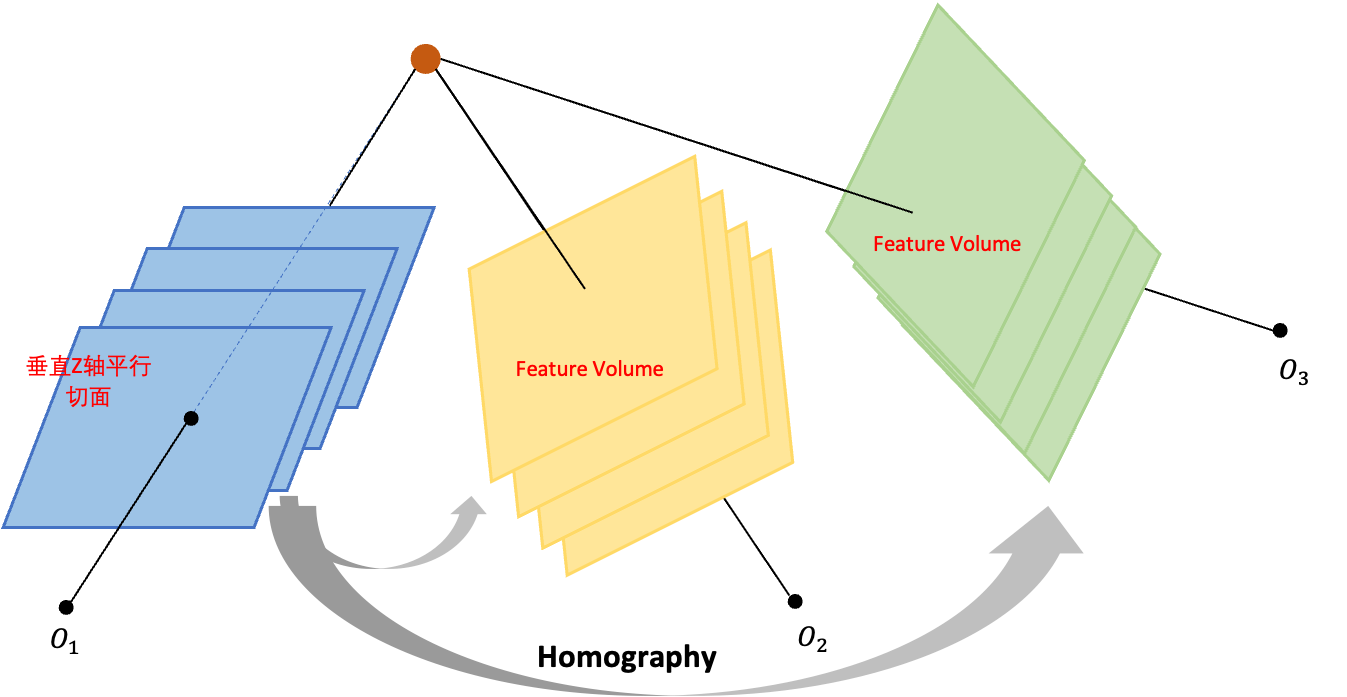
\includegraphics[width=\textwidth]{images/fronto.png}
		\end{center}
		\caption{相机1将场景按深度切片称为\textbf{Fronto parallel},分别投影到相机2,3像素平面,形成\textbf{Feature Volume}}
	\end{figure}

\subsection{目标相机的作用}

	目标相机对预测参考图像的深度有什么帮助?我是这么认为的,因为世界坐标系选为参考相机的坐标系,如果参考图像上有一个点深度为$d$,那么其他相机看到这个点深度也应该为$d$,也就是用目标图像的特征预测出的深度也应该为$d$。\\

	因此,如果一个点的深度在各个相机下预测正确,那么方差就会很小,否则方差会变大,这是作者认为\textbf{Cost Volume}有作用的原因。\\

	把\textbf{Feature Volume}的平均作为回归目标也是可行的,但作者在消融实验提到效果不如方差,这里是个玄学。\\

	提升目标图片数量,预测效果也会提升,作者实验过5张图片效果好于2张。能提升预测效果的图片是那些与目标相机姿态差距不是很大的图片,所以这个数量也是有上限的。

\subsection{单应变换的作用}
	MVSNet工作重点便是单应变换,主要体现在:
	\begin{itemize}
		\item 通过单应变换把场景切面变换到目标相机像素坐标系
		\item 单应变换可求导,使得变换过程可训练
	\end{itemize}

	然而,变换切面通过增广矩阵的逆变换即可,矩阵变换本身可求导,顺便包含了第二点。\\

	虽然全文都在介绍单应矩阵,实现实际完全不需要这个概念,更不需要那些复杂的推导,是不是有点讽刺!\\

	需要考虑下面两个问题,对单应变换的影响,
	\begin{itemize}
		\item 不同深度的切面通过单应变换产生的像素值会有多大的差异?
		\item 单应变换产生的新坐标如何跟目标特征图结合生成新的特征图?
	\end{itemize}

	\subsubsection*{深度对像素坐标的影响}
	对第一个问题,单应矩阵$H$可以简化为,

	\begin{align*}
		H_d= K^{\prime}\left(R + T\mathbf{n}_d^T\right)K^{-1} &= \mathbf{A} +\frac{1}{d}\mathbf{B}\\
		&= \begin{bmatrix}
			\mathbf{A}_1 + \frac{1}{d}\mathbf{B}_1\\
			\mathbf{A}_2 + \frac{1}{d}\mathbf{B}_3\\
			\mathbf{A}_3 + \frac{1}{d}\mathbf{B}_4
		\end{bmatrix}
	\end{align*}

	$\mathbf{A}=K^\prime R K^{-1},\mathbf{B}=K^{\prime}T\mathbf{n}^TK^{-1}$,只有$d$是变量,
	$$
		p^\prime(d) = H_d p = \begin{bmatrix}
			\left(\mathbf{A}_1 + \frac{1}{d}\mathbf{B}_1\right)p\\
			\left(\mathbf{A}_2 + \frac{1}{d}\mathbf{B}_3\right)p\\
			\left(\mathbf{A}_3 + \frac{1}{d}\mathbf{B}_4\right)p
		\end{bmatrix}
	$$

	$p^\prime$的欧式坐标$p^\prime_e$为,
	$$
		p^\prime_e(d) = \left(
			\frac{\left(\mathbf{A}_1 + \frac{1}{d}\mathbf{B}_1\right)p}{\left(\mathbf{A}_3 + \frac{1}{d}\mathbf{B}_3\right)p},
			\frac{\left(\mathbf{A}_2 + \frac{1}{d}\mathbf{B}_3\right)p}{\left(\mathbf{A}_3 + \frac{1}{d}\mathbf{B}_3\right)p}
		\right)^T
	$$

	$$
		p^\prime_e(\infty) = \lim_{d\rightarrow \infty}p^\prime_e(d) = \left(
			\frac{\mathbf{A}_1p}{\mathbf{A}_3p},
			\frac{\mathbf{A}_2p}{\mathbf{A}_3p}
		\right)^T
	$$

	$$
		p^\prime_e(0) = \lim_{d\rightarrow 0}p^\prime_e(d) = \left(
			\frac{\mathbf{B}_1p}{\mathbf{B}_3p},
			\frac{\mathbf{B}_2p}{\mathbf{B}_3p}
		\right)^T
	$$	

	深度$d$的确影响投影的$u,v$坐标,且输出在$p^\prime_e(0)$和$p^\prime_e(\infty)$之间。\\

	但因为在两端存在极限,所以$d$在一定的区间内变化,对$u,v$才能有显著的影响,
	
	\subsubsection*{变换特征映射}
		现在考虑第二个问题,参考相机和目标相机像素平面分辨率为$120 \times 160$,超出这个区间的变换坐标怎么处理?\\

		MVSNet的是根据最大坐标值,$u^\prime = u/119, v^\prime = v/159$(坐标从0开始)后变换到$[-1,1]$,对超出此区间的坐标一律忽略。\\

		目标特征图的左上角对应$(-1,-1)$,右下角对应$(1,1)$,根据$(u^\prime, v^\prime)$的值查找特征图上对应的点(连续值),并根据周围四个坐标(离散值)做双线性插值计算具体对应值。\\

		显然,考相机和目标相机的分辨率即使不同,也不影响这个插值过程。\\

		如果超出$(120,160)$的坐标都被忽略,是否会降低学习效果?\\

		这里实际隐含一个约束,要求两个相机应该能看到尽量多的共同点,这通过图像对的选择策略来实现,称为\textbf{视角选择}。

\subsection{视角选择}
	
	\begin{figure}[H]
		\begin{minipage}[t]{0.48\linewidth}
			\centering
			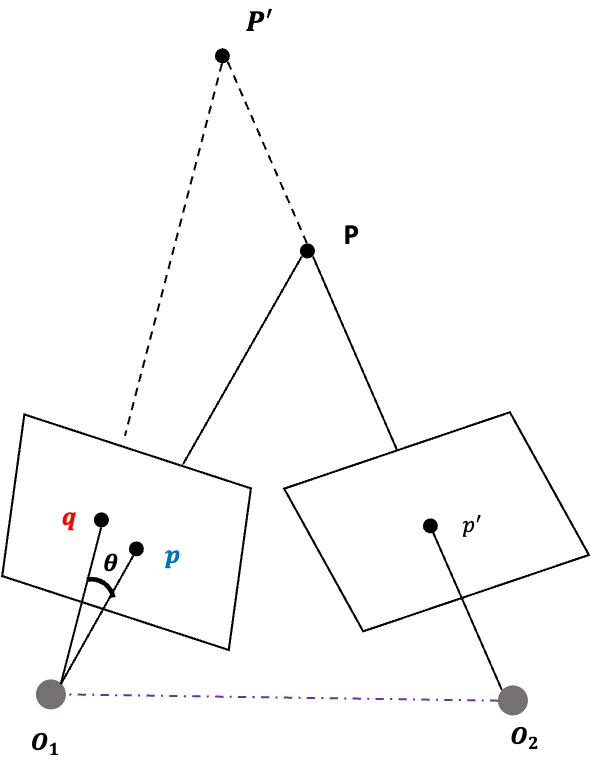
\includegraphics[width=\textwidth]{images/baseline_error.png}
			\caption{基线太小,重建误差较大}
		\end{minipage}		
		\begin{minipage}[t]{0.52\linewidth}
			\centering
			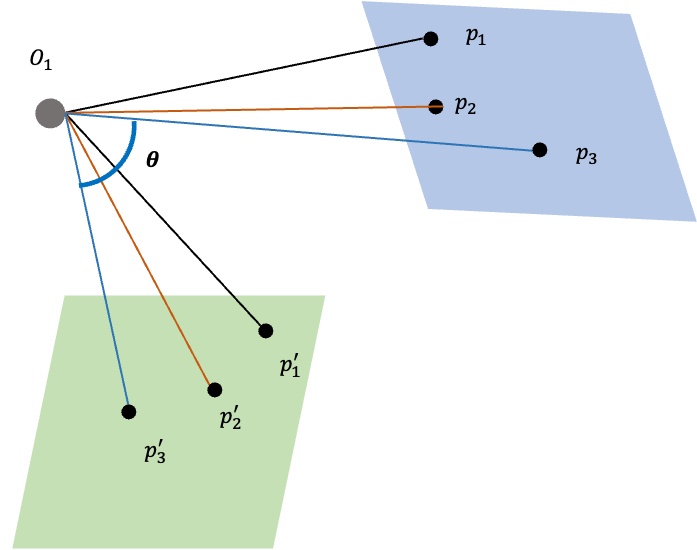
\includegraphics[width=\textwidth]{images/track_filter.png}
			\caption{通过Track过滤小基线视角}
		\end{minipage}			
	\end{figure}

	图一小基线的场景,如果$p^\prime$误匹配$q$,$p,q$虽然只偏离了一个小角度$\theta$,重建的$P^\prime$与$P$误差也很大。\\

	反之,大基线场景会产生遮挡,极大减少可重建点数。MVSNet给出下面的评分机制来选择合适的图像对,

	$$
		\theta_{ij} = (180/\pi)\arccos\left(
			(\mathbf{c}_i - \mathbf{p})
			\cdot
			(\mathbf{c}_j - \mathbf{p})
		\right)
	$$

	$\theta_{ij}$为点对夹角,计算方法是:将像素坐标投影回世界坐标系,以第一个相机的光心为原点计算内积的反余弦(图二);\\

	\textit{相机内参和像素坐标都已知,这个过程是没问题的。}\\

	通过下面分段函数把$\theta_{ij}$拟合为打分,

	$$
		\mathcal{G}(\theta) = 
		\begin{cases}
			\exp\left(
				-\frac{(\theta-\theta_0)^2}{2\sigma_1^2}
			\right), \theta \leq \theta_0\\
			\exp\left(
				-\frac{(\theta-\theta_0)^2}{2\sigma_2^2}
			\right), \theta > \theta_0\\
		\end{cases}
	$$

	\begin{figure}[H]
		\begin{center}
			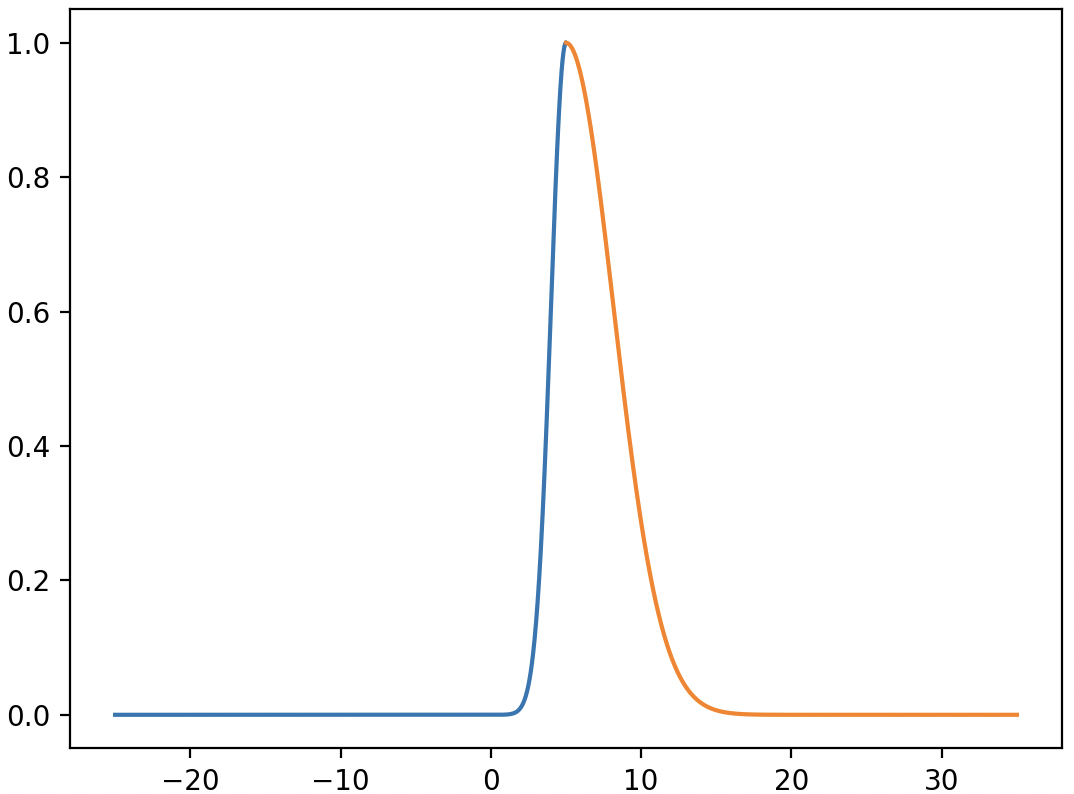
\includegraphics[width=0.9\textwidth]{images/piece_gaussian.png}
		\end{center}
		\caption{分段高斯函数,$\theta_0=5, \sigma_1 = 1, \sigma_2 = 10$}
	\end{figure}

	该函数对小基线惩罚更大,夹角小于$5$度,走小方差分支,下降更快;大于5度,走大方差分支,下降平稳一些。\\

	最终图像对打分,
	$$
		s_{ij} = \sum_{\mathbf{p}}\mathcal{G}\left(\theta_{ij}(\mathbf{p})\right)
	$$

	匹配点对越多,且夹角不小于5度,则图像之间打分越高。

\subsection{实现细节}
	MVSNet将$1200 \times 1600$的原图下采样到$800 \time 600$,从中心crop出$512 \times 640$作为输入,经过特征提取后生成$128 \times 160 \times 32$的特征图。\\

	输出为参考图的深度值,GroundTruth也是参考图的深度值,均为$128 \times 160$。 处理分几个步骤,

	\begin{itemize}
		\item 每次输入3张图,一张为参考,2张目标,经过特征提取后,得到三个$128 \times 160 \times 32$的特征图
		
		\item 采用192个深度单位,通过单应变换将参考坐标变换到两个目标相机姿态下

			\textit{作者原始实现用了复杂的单应矩阵,非常繁琐;pytorch版本用了增广变换矩阵,非常简洁}

		\item 根据坐标变换得到两个$192 \times 128 \times 160 \times 32$的特征图,如上节描述

			\textit{按深度方向,从425mm到935mm,按2mm间隔离散成192个像平面}

		\item 连同参考特征图一起,计算三个\textbf{Feauture Volume}的方差,得到\textbf{Cost Volume};进行3D卷积,通过softmax沿着深度方向作概率归一化,结果为\textbf{Probability Volume},维度为$192 \times 128 \times 160$

		\item 沿\textbf{Probability Volume}深度方向计算深度期望值,得到维度为$128 \times 160$的深度特征图,
			$$
				D = \sum_{d = d_{min}}^{d_{max}} d \times \mathbf{P}(d)
			$$

			论文中提到,这一步实际想对\textbf{Probability Volume}作一个$\arg\max$操作,选出当前位置最可能的深度值,但是$\arg\max$无法求导,无法进行梯度回传,所以用soft $\arg\max$(原文说成是soft $\arg\min$)。

			\textit{所谓soft $\arg\max$实际就是利用了$softmax$逼近$\arg\max$的特性,以此来代替$\arg\max$\footnote{\url{https://en.wikipedia.org/wiki/Softmax_function}}}

		\item 通过$L_1$回归参考图的深度值;这里只有参考图的深度值为GroundTruth,src图的深度值未使用。
	\end{itemize}

	在增量SfM方法中,一次考虑所有图像,通过反投影距离进行优化,得到整个场景的点云;但在具体实现中,至少被三个相机看到的点,才能重建出点云;\\

	MVSNet中,训练的时候只是用了3张图片,但可以推断出参考图像上所有点的深度信息;在后处理时需要把图片两两输入,构建整个场景的点云。\\

	SfM的依赖图像之间的对应点对,具体会通过SIFT特征或深度学习的方法去构建对应关系;这一步实际也会引入很多匹配噪音,尤其对一些纹理较少的图像,能计算出的匹配点较少。\\

	MVSNet没有这一步处理,对应关系已经隐含在深度预测中,能匹配的点对,看到的深度也应该一样。\\

	事实证明,通过隐式特征构建对应关系,远远好于在RGB空间用显式特征构建对应关系。

\subsection{后处理}
	主要是对深度作两种过滤,

	\begin{itemize}
		\item \textbf{\textit{photometric约束}} \\

		对\textbf{Probability Volume}中概率小于0.8的点进行过滤;对噪音点不同的相机做出的判断方差会比较大,从而回归出的概率会变小

		\item \textbf{\textit{geometric约束}} \\
			
			点对$p,p^\prime$,以$p$图为参考图预测出深度值$d$;以$p^\prime$为参考图,预测出深度值$d^\prime$\\

			将$p^\prime$以深度$d^\prime$反投影到第一个视图,得到$p_{reproj}$,及对应的深度$d_{reproj}$

		\begin{align*}
			&\vert p - p_{reproj}| < 1\\
			&\frac{\vert d - d_{reproj}\vert}{d} < 0.01
		\end{align*}
		
		使得像素误差在1像素内,深度误差在1\%以内,文中提到这种约束至少在3视图上执行,如此同一点会有很多个重投影深度,取平均作为当前点的最终深度。
	\end{itemize}

\subsection{深度图融合}
	将不同视觉的深度图融合成场景点云,MVSNet采用“Real-time visibility-based fusion of depth maps”\footnote{\url{https://people.inf.ethz.ch/pomarc/pubs/MerrellICCV07subm.pdf}}的方法,看了下就是基于简单的遮挡规则来过滤一些不置信的点。\\

	这个文章也是作者的,虽然文中引用了自身,但code是在他人基础上改的,思路是下面第一篇。。。

	\begin{itemize}
		\item  Massively parallel multiview stereopsis by surface normal diffusion\footnote{\url{https://www.cv-foundation.org/openaccess/content_iccv_2015/papers/Galliani_Massively_Parallel_Multiview_ICCV_2015_paper.pdf}}
		\item Pixelwise view selection for unstructured multi-view stereo(COLMAP)\footnote{\url{https://demuc.de/papers/schoenberger2016mvs.pdf}}
		\item Structure-from-Motion Revisited\footnote{\url{https://openaccess.thecvf.com/content_cvpr_2016/papers/Schonberger_Structure-From-Motion_Revisited_CVPR_2016_paper.pdf}}
	\end{itemize}

	后两篇文章是COLMap的基础,MVSNet也有间接参考。

\subsection{问题\&改进}
	为什么要将场景切成192片,作单应变换去构建Cost,而不是直接通过基础矩阵变换构建Cost?\\

	单应变换是传统处理常用的手段,这个文章发表比较早,受传统MVS影响比较大,可能当时还没有建立端到端的思路,或者是端到端没做出效果。\\

	切片思路得假设目标场景最大最小距离,切片多了影响计算性能,并且有很多无意义的切片;切片少了又影响精度,对此"Cascade Cost Volume for High-Resolution Multi-View Stereo and Stereo Matching"\footnote{\url{https://arxiv.org/abs/1912.06378}}这个文章专门提了一些切片的优化方法,后面我们再细说。

\section{训练集结构}
	
	\subsection*{DTU数据集} 
		mvsnet用的是DTU数据集,DTU数据集通过移动的机械臂在$49$或$64$个位置,用$7$种光照,通过结构光扫描了$124$个场景,生成$1200 \times 1600$像素的图片及对应的点云信息。\\

		因此,每个场景有$49 * 7 = 343$张照片,整体数据集包含$42532$张照片及对应的点云信息。因为机械臂移动受到严格控制,所以每张图片都有对应的高精度相机参数。\\

		mvsnet训练集用了$79$个场景,共计$27097$张图片;测试集用了$22$个场景,共计$7546$张图片。
	
	\subsection*{深度信息}
		MVSNet的输入的是每个点的深度,通过泊松表面重建,将DTU数据集的点云转变为mesh,计算出每个像素点对应的深度信息。

	\subsection*{数据集结构}
		\begin{itemize}
			\item mvs{\_}training$\slash$dtu$\slash$Cameras$\slash$pair.txt 记录了$49$个位置,每个位置的照片与其他$10$张照片的匹配程度;注意这个pair内容与场景无关,仅与相机位置有关。因为相机位置受到精准控制,所以通过空间关系可以描述出位置之间的差异。

			\item mvs{\_}training$\slash$dtu$\slash$Cameras{\_}train$\slash$000000\{YY\}{\_}cam.txt 存放相机内外参数及尺度缩放信息

			\item mvs{\_}training$\slash$dtu$\slash$Rectified$\slash$scan\{XX\}{\_}train 训练样本,XX为场景编号
				\begin{itemize}
					\item rect{\_}0\{YY\}{\_}\{Z\}{\_}r5000 为场景scanXX对应的图片,YY为相机位置编号$ 1 \sim 49$,Z为光照强度编号$0 \sim 6$
				\end{itemize}

			\item mvs{\_}training$\slash$dtu$\slash$Depths$\slash$scan\{XX\}{\_}train$\slash$
				\begin{itemize}
					\item depth{\_} map{\_}00\{YY\}.pfm 场景scanXX对应相机位置YY($0 \sim 48$)的深度图,格式为pfm
					\item depth{\_} map{\_}00\{YY\}.png 深度图的可视化
				\end{itemize}
			
		\end{itemize}	